%------------------------- CONCEPT 1 -------------------------%
\subsection{Concept 1 - Linkage}

This concept uses the basic principle of a rotary-to-linear linkage by imposing movement restriction. The rotary movement is created by the motor, which is connected to the crankshaft. The rod connected to the crankshaft is modified to allow vertical sliding and rotation around the fixed guiding pin. The crankshaft mechanism allows for the leg/connecting rod to be lifted off the ground. The guiding pin restricts certain movements of the connecting rod, creating a pendulum movement. By combining both mechanisms, the connecting rod is moved front to back on the ground and back to front off the ground. By combining the pattern for each leg of the robot, a walking sequence is achieved. Figure \ref{fig:concept1_linkage} shows the concept of the mechanism.

\begin{figure}[H]
    \centering
    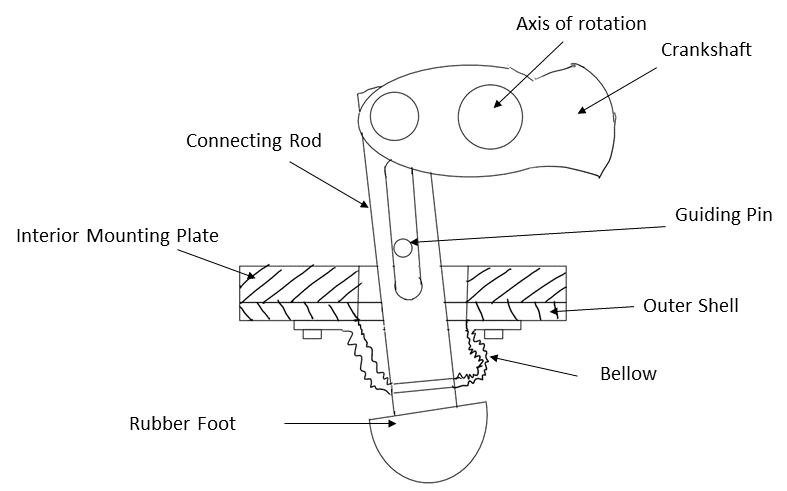
\includegraphics[width=0.8\textwidth]{img/C1/Concept.PNG}
    \caption{Linkage Side View - Concept}
    \label{fig:concept1_linkage}
\end{figure}

In this concept, all legs are powered by their respective gearmotor. The shaft assembly from the gearmotor to the crankshaft is shown in Figure \ref{fig:concept1_Crankshaft}. The gearmotor is face/flange mounted on an L bracket mounted to the structural mounting plate (not shown in figure). The crankshaft is coupled to the gearmotor using a setscrew shaft coupler, and the crankshaft is supported on the opposite end of the gearmotor by a pillow mounted bearing.

\begin{figure}[H]
    \centering
    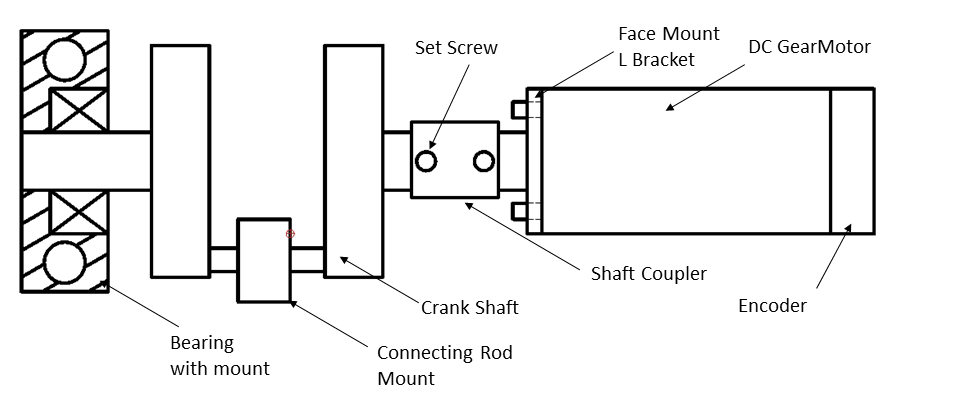
\includegraphics[width=0.8\textwidth]{img/C1/Crankshaft.PNG}
    \caption{Linkage Top View - Motor Crankshaft Assembly}
    \label{fig:concept1_Crankshaft}
\end{figure}

The connecting rod is the leg/limb of the robot. It is coupled to the crankshaft using typical mounting procedures. As shown in Figure \ref{fig:concept1_ConnectingRod}, the connecting rod is mounted on the crankshaft using two bolts and nuts and will rotate around the crankshaft through the use of bushings. 

\begin{figure}[H]
    \centering
    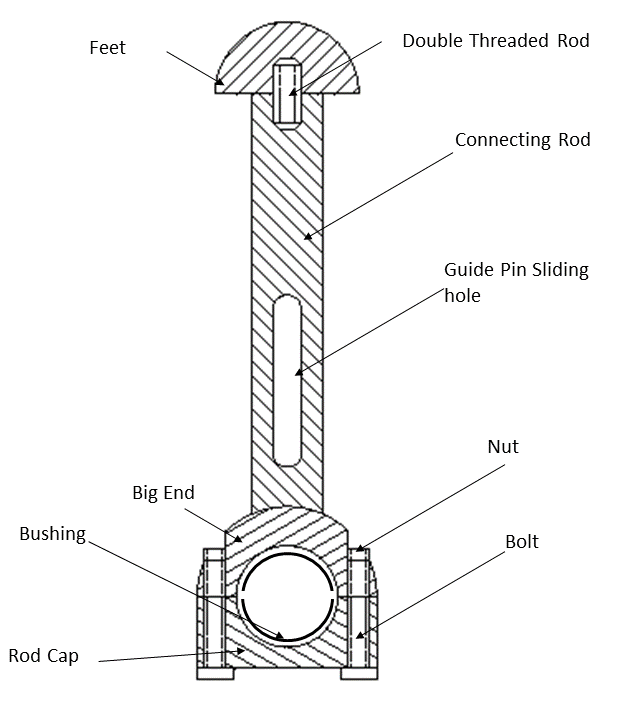
\includegraphics[width=0.6\textwidth]{img/C1/ConnectingRod.PNG}
    \caption{Linkage Side View - Connecting Rod}
    \label{fig:concept1_ConnectingRod}
\end{figure}

The guiding pin is the critical component in this concept as it enables the walking pattern and will be subject to multiple forces. The guiding pin is inserted through the sliding hole and fastened using the threaded end to mounting blocks. The sliding hole enables the pin to be supported on both end avoiding a cantilever support. The pin is also mounted with a spacer and bearing to facilitate rotation and reduce wear on the connecting rod. A top view of the guiding pin assembly is shown in Figure \ref{fig:concept1_GuidingPinTop} and a side view of the guiding pin is shown in Figure \ref{fig:concept1_GuidingPinSide}. The Figure \ref{fig:concept1_GuidingPinSide} also shows the mounting procedure for the bellow, the mounting plate and the exterior material. The mounting plate is a sheet metal acting as structural element to the chassis of the robot and will support all components. All major equipment are mounted on the mounting plate. The exterior material, most likely polycarbonate due to its weather resistant properties, will be an outer shell protecting electronic and mechanical components from water, salt and other destructive particles. The bellow is face mounted through the exterior material and through the mounting plate to allow for better structural integrity between the mounting plate and the outer shell. The other end of the bellow will be elastically tightened to the connecting rod between the feet and the guide pin sliding hole.  

\begin{figure}[H]
    \centering
    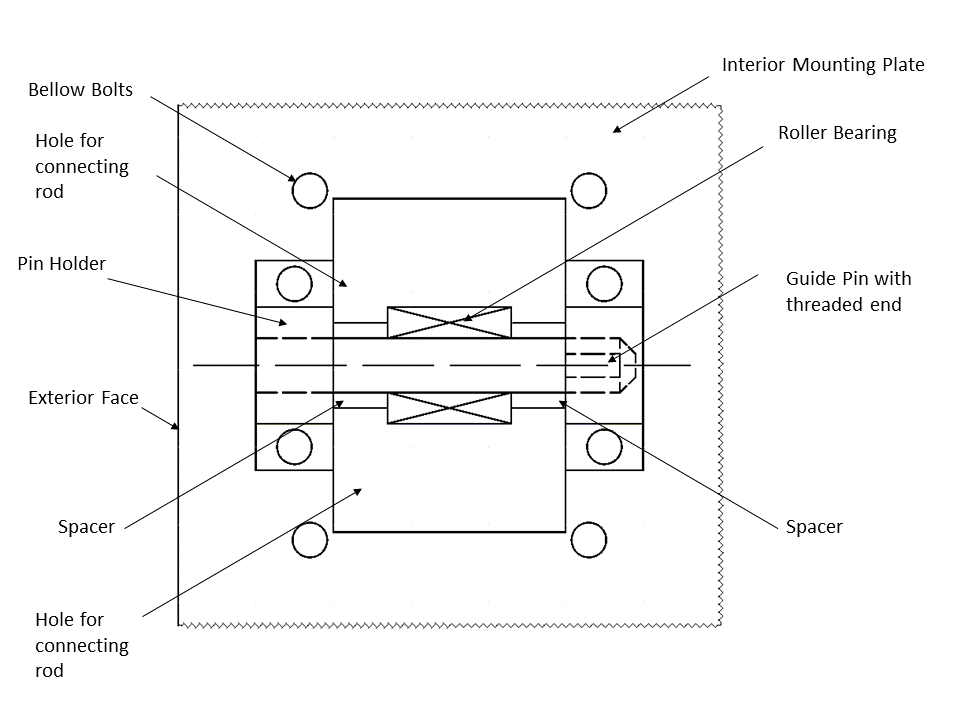
\includegraphics[width=0.8\textwidth]{img/C1/GuidingPin_Top.PNG}
    \caption{Linkage Top View - Guiding Pin Mount Assembly}
    \label{fig:concept1_GuidingPinTop}
\end{figure}

\begin{figure}[H]
    \centering
    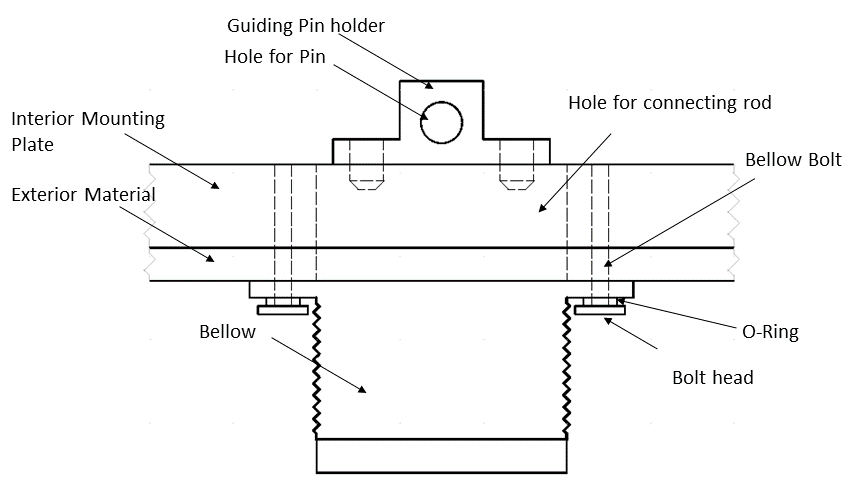
\includegraphics[width=0.8\textwidth]{img/C1/GuidingPin_Side.PNG}
    \caption{Linkage Side View - Guiding Pin and Bellow Mount Assembly}
    \label{fig:concept1_GuidingPinSide}
\end{figure}

The case's (or outer shell) purpose is to protect all equipment and components from exterior activities. Access to the components is required as they may be subject to maintenance. The case is thus separated in two parts, the top and bottom as shown in Figure \ref{fig:concept1_CaseSide}. Both parts are sealed using a gasket as shown in \ref{fig:concept1_CaseTop} and they are fastened together using multiple bolts surrounding the casing. Figure \ref{fig:concept1_CaseTop} also shows the holes and bolt mounting location of the bellows on the outer shell case.

\begin{figure}[H]
    \centering
    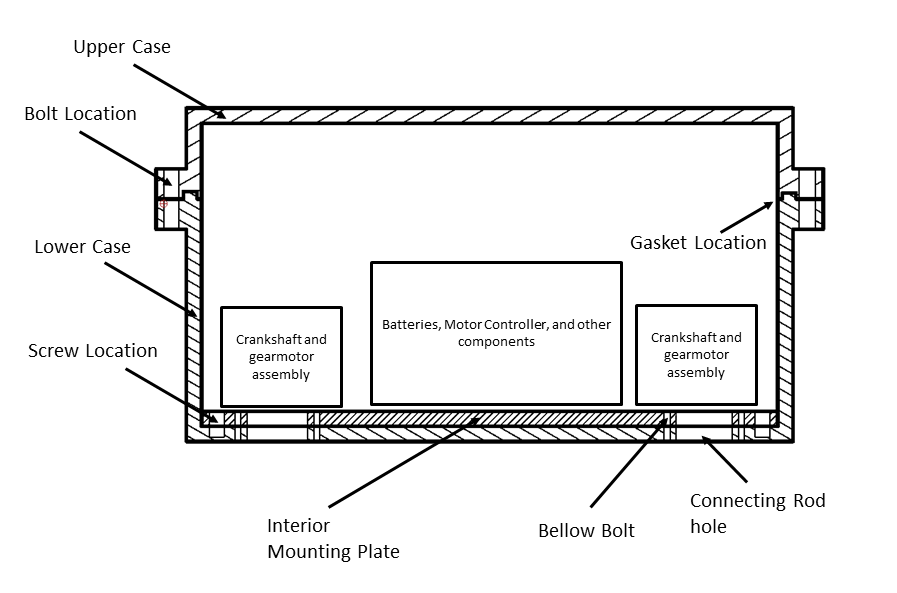
\includegraphics[width=0.8\textwidth]{img/C1/Case_Side.PNG}
    \caption{Linkage Side View - Water and Weather proof casing}
    \label{fig:concept1_CaseSide}
\end{figure}

\begin{figure}[H]
    \centering
    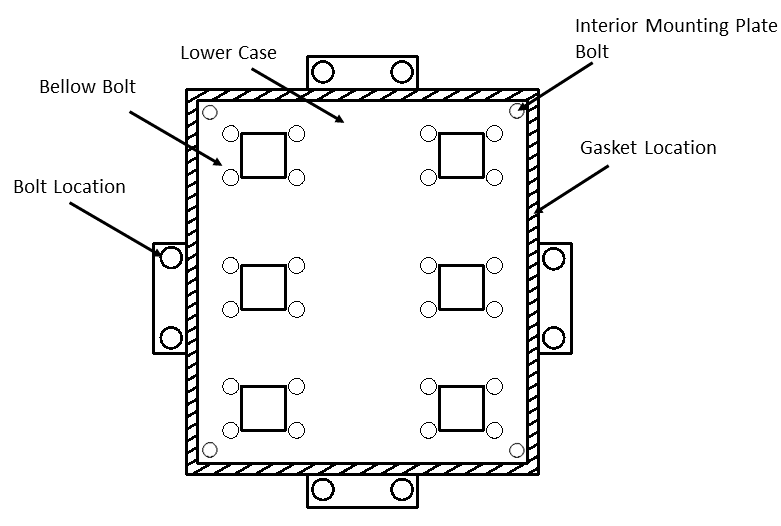
\includegraphics[width=0.8\textwidth]{img/C1/Case_Top.PNG}
    \caption{Linkage Top View - Water and Weather proof casing}
    \label{fig:concept1_CaseTop}
\end{figure}

To achieve a stable and reliable locomotion, the robot will be equipped with six legs. The mounting plate must mount all components required for the locomotion, and power system. The Figure \ref{fig:concept1_MountingPlate} depicts the layout of the equipment and their respective mounting holes. The robot will rotate using the same principle as a tracked tank, such that on one side the leg will complete the walking pattern more quickly than on the other side.

\begin{figure}[H]
    \centering
    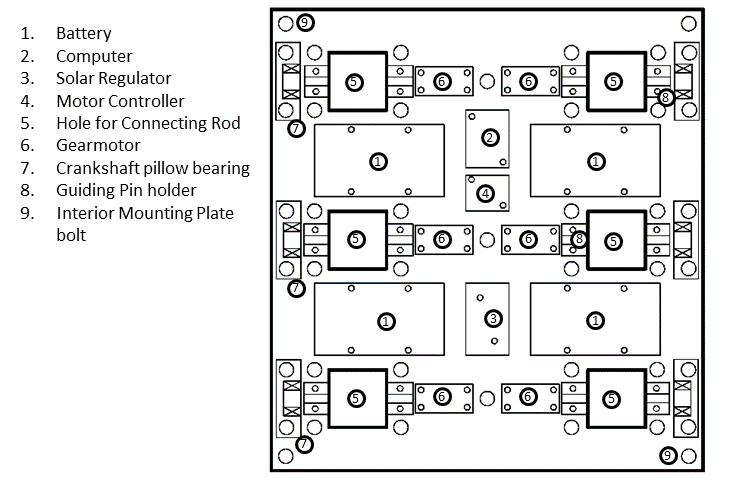
\includegraphics[width=\textwidth]{img/C1/MountingPlate.png}
    \caption{Linkage Top View - Structural Mounting Plate}
    \label{fig:concept1_MountingPlate}
\end{figure}



%------------------------- CONCEPT 2 -------------------------%
\subsection{Concept 2 - Crab} \label{subsec:crab}

The second concept is based on the movement of sideways-walking crabs. This idea was further developed to include legs at the front and back of the chassis instead of at the sides, as shown in Figure \ref{fig:crab_top}. The legs are thus making pulling and pushing motions. There are five legs in total, as a space is left at the front to accommodate the waste collection system. 

\begin{figure}[H]
    \centering
    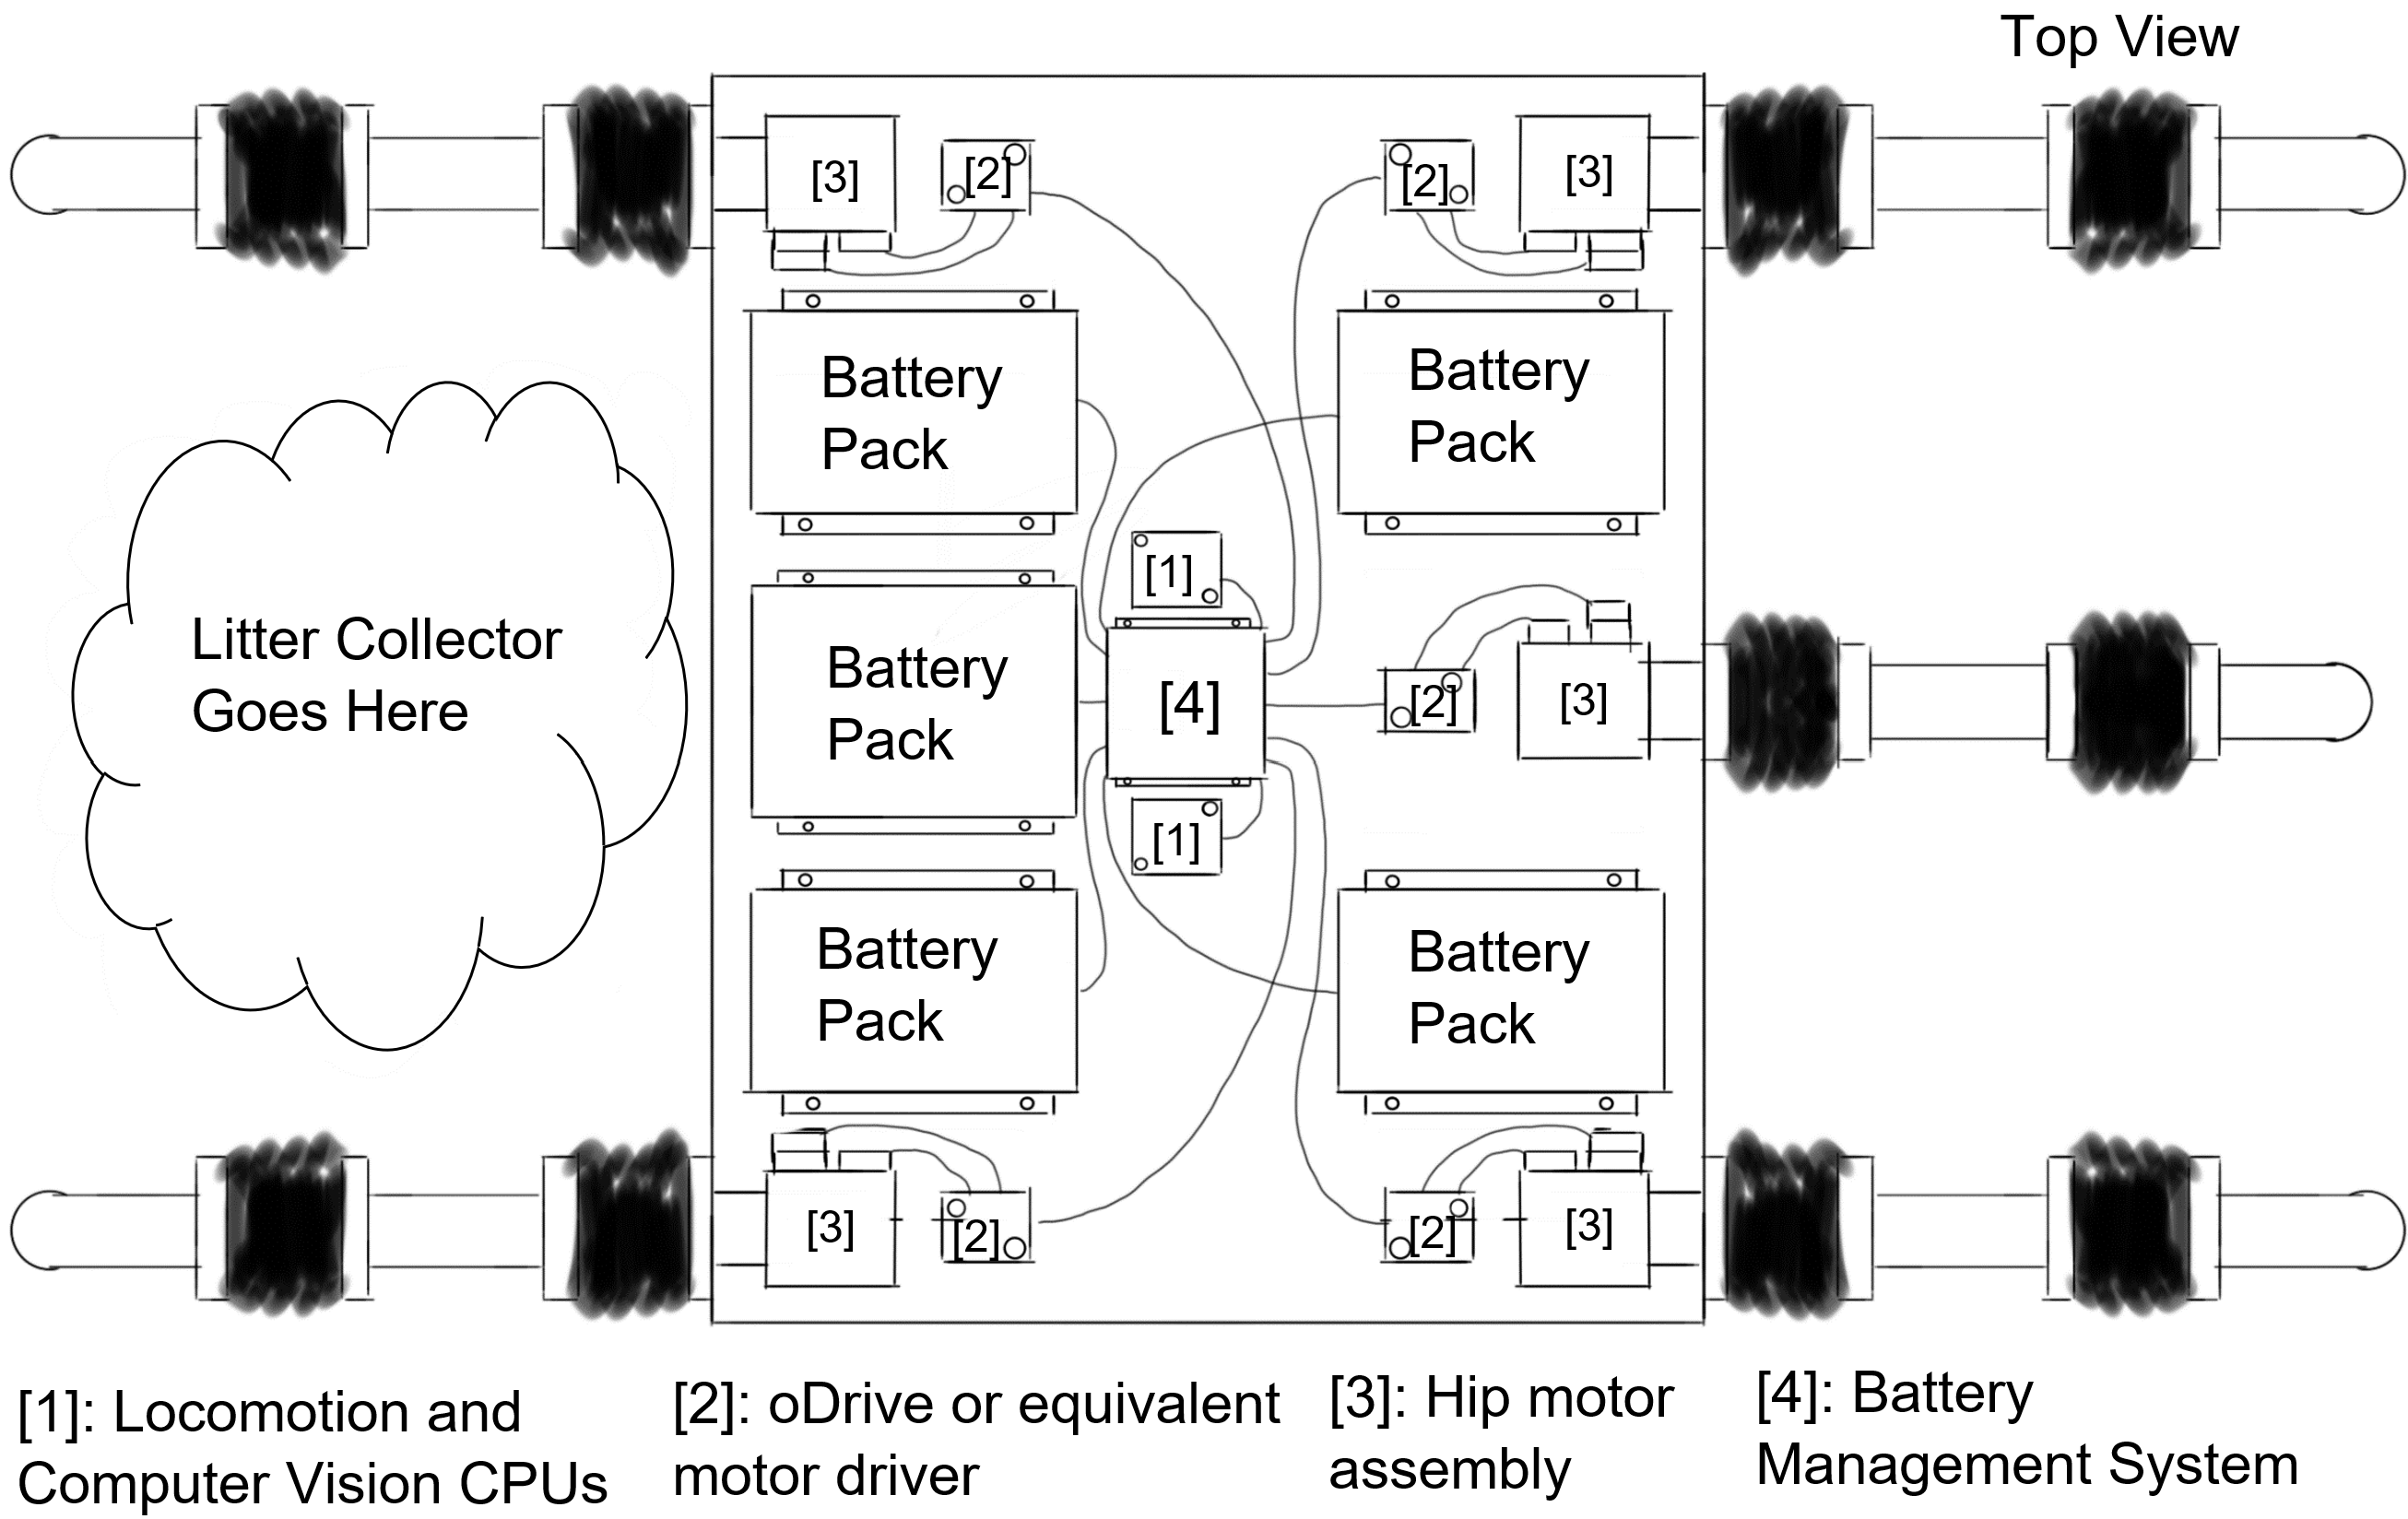
\includegraphics[width=\textwidth]{3_DesignConcepts/img/Crab/crab_top_view.png}
    \caption{Crab Top View - Concept}
    \label{fig:crab_top}
\end{figure}

Figure \ref{fig:crab_top} also shows the layout of the various electrical components within the chassis. Five battery packs are managed by the central Batter Management System that will then distribute the power to individual motor controllers. In case a battery pack dies, the system should be able to keep running fully with four, three or even one battery pack at reduced run times. The segmentation also allows for better weight distribution.
One computer is responsible for locomotion and general computing and the second is used for computer vision/machine learning algorithms to identify litter and obstacles.

Figure \ref{fig:crab_leg} shows a side view of a full leg. The legs have two DOF: one up and down rotating motion at the hip, and another one at the knee. This allows for extension of the leg and up and down rotation. Both motors (here Maxon Motor EC 60 100 W, shown in Appendix \ref{app:data_sheets}) controlling the motion are located inside the chassis, with a belt drive mechanism being used to control the knee. This will reduce the inertia of the leg and the use of electronics outside the chassis. There is no rotating motion on the legs which would cause them to be able to turn the robot left and right. However, this is possible by having the legs on one side walking faster than the other, or having one side walking forwards while the other walks backwards. This method has been used in robots before, such as Stanford Doggo, and is also the method by which tanks turn on themselves \cite{kau_stanford_2019}.

Molded bellow covers are being used to cover the openings at the knee and the chassis. Both the clamping (cuff) mounting method (at the knee) and the flange mounting method (at the hip) are shown as possible options. As the bellows are rectangular/square, the flange mounting is more readily available, and thus was used for the cost estimate (rectangular cuff ends might require a custom bellow). The mounting of a square flange type bellow at the knee would be similar to the method shown in concept 3. The shin linkage has a corner in order to reduce the angle for the bellow. The linkages representing the thigh and shin may vary in length, thickness and material, depending on the results of the kinetic analysis. A carbon fiber square tubing was used for the linkages as a preliminary material for the cost assessment. Mechanical properties are shown in Appendix \ref{app:data_sheets}

\begin{figure}[H]
    \centering
    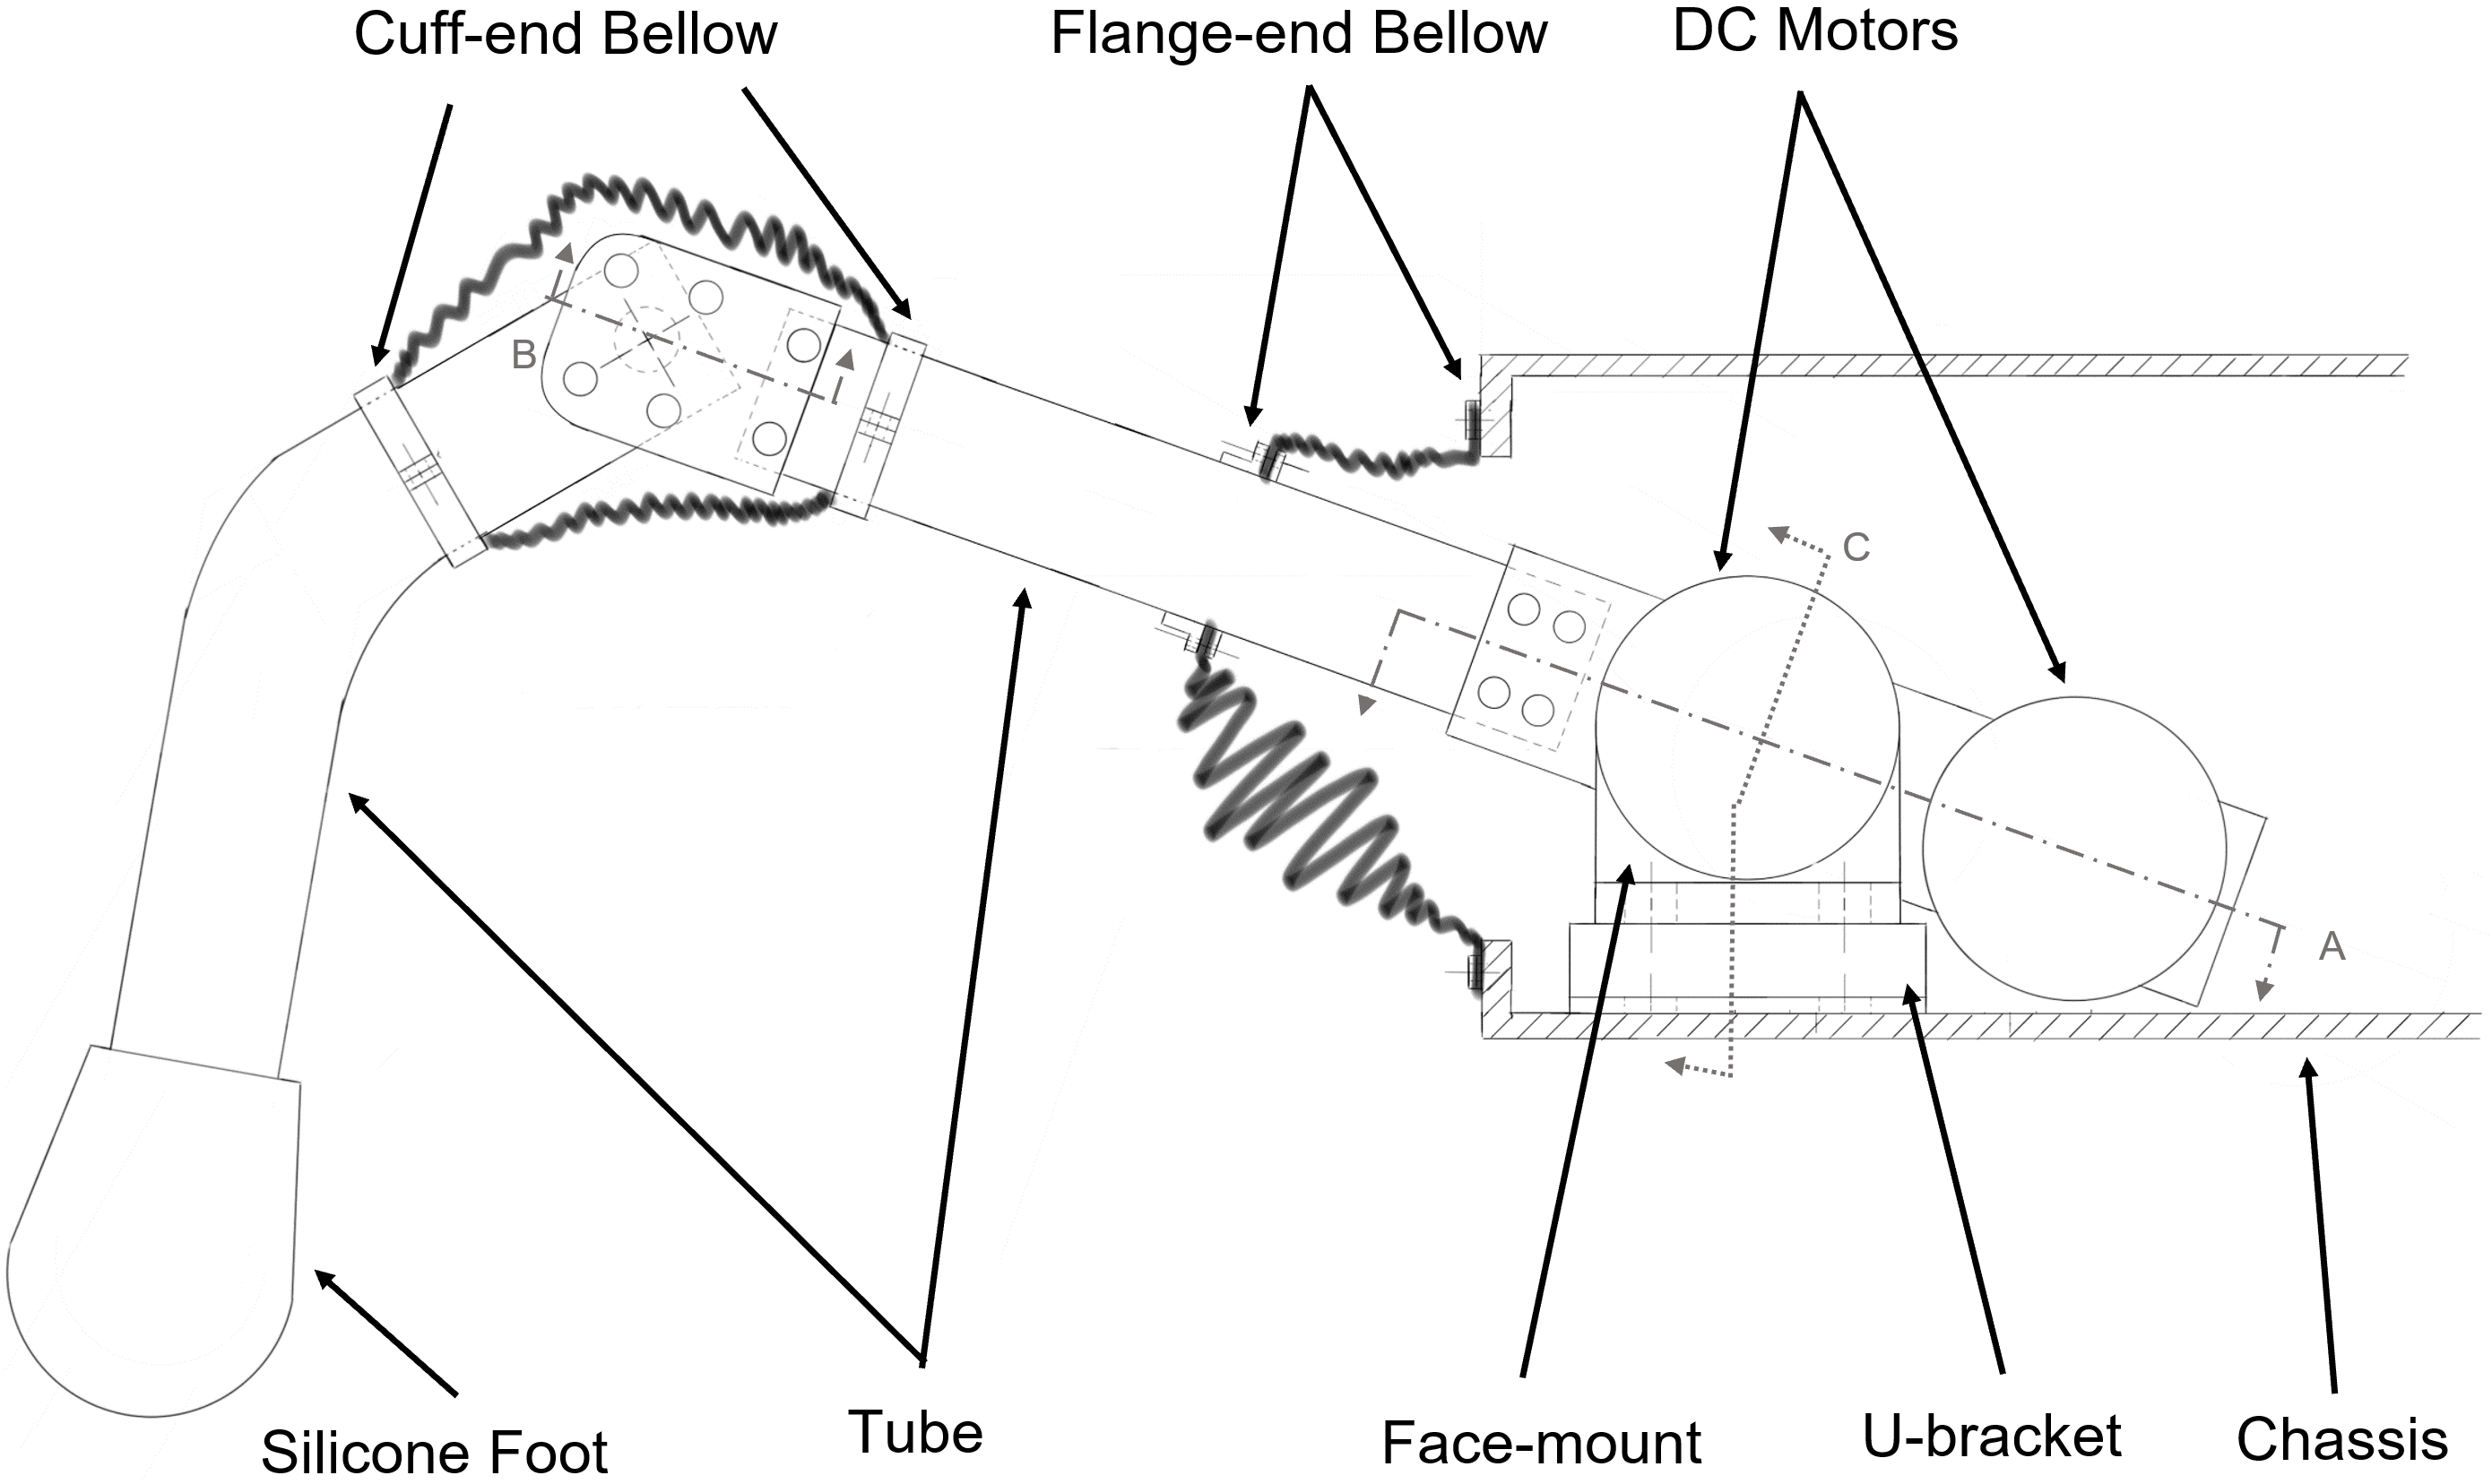
\includegraphics[width=\textwidth]{3_DesignConcepts/img/Crab/crab_leg.png}
    \caption{Crab Side View - Full Leg}
    \label{fig:crab_leg}
\end{figure}

Figures \ref{fig:crab_hip} and \ref{fig:crab_hip_cut} show the detailed concept for the hip joint (Sections A and C as per Figure \ref{fig:crab_leg}).
The leftmost motor and gearbox in Figure \ref{fig:crab_hip} are attached directly to the leg and turn it from the hip; the second motor (on the right) turns the pulley, in turn manipulating the knee joint.
Figure \ref{fig:crab_hip_cut} illustrates the bracketing not shown in Figure \ref{fig:crab_hip}, that connects the hip assembly to the chassis.
It is cut perpendicular to the cut shown in Figure \ref{fig:crab_leg}.

The gearbox is a Harmonic Drive CSD series component set, allowing for high torque in a very thin form-factor \cite{harmonic_drive_csd-2a_nodate}. Their outer diameter varies between 50 and 170 mm, thickness between 11 and 33 mm, and output torques between 3.7 and 370 Nm.
Their primary weakness is low efficiency (shown in Appendix \ref{app:data_sheets}).

\begin{figure}[H]
    \centering
    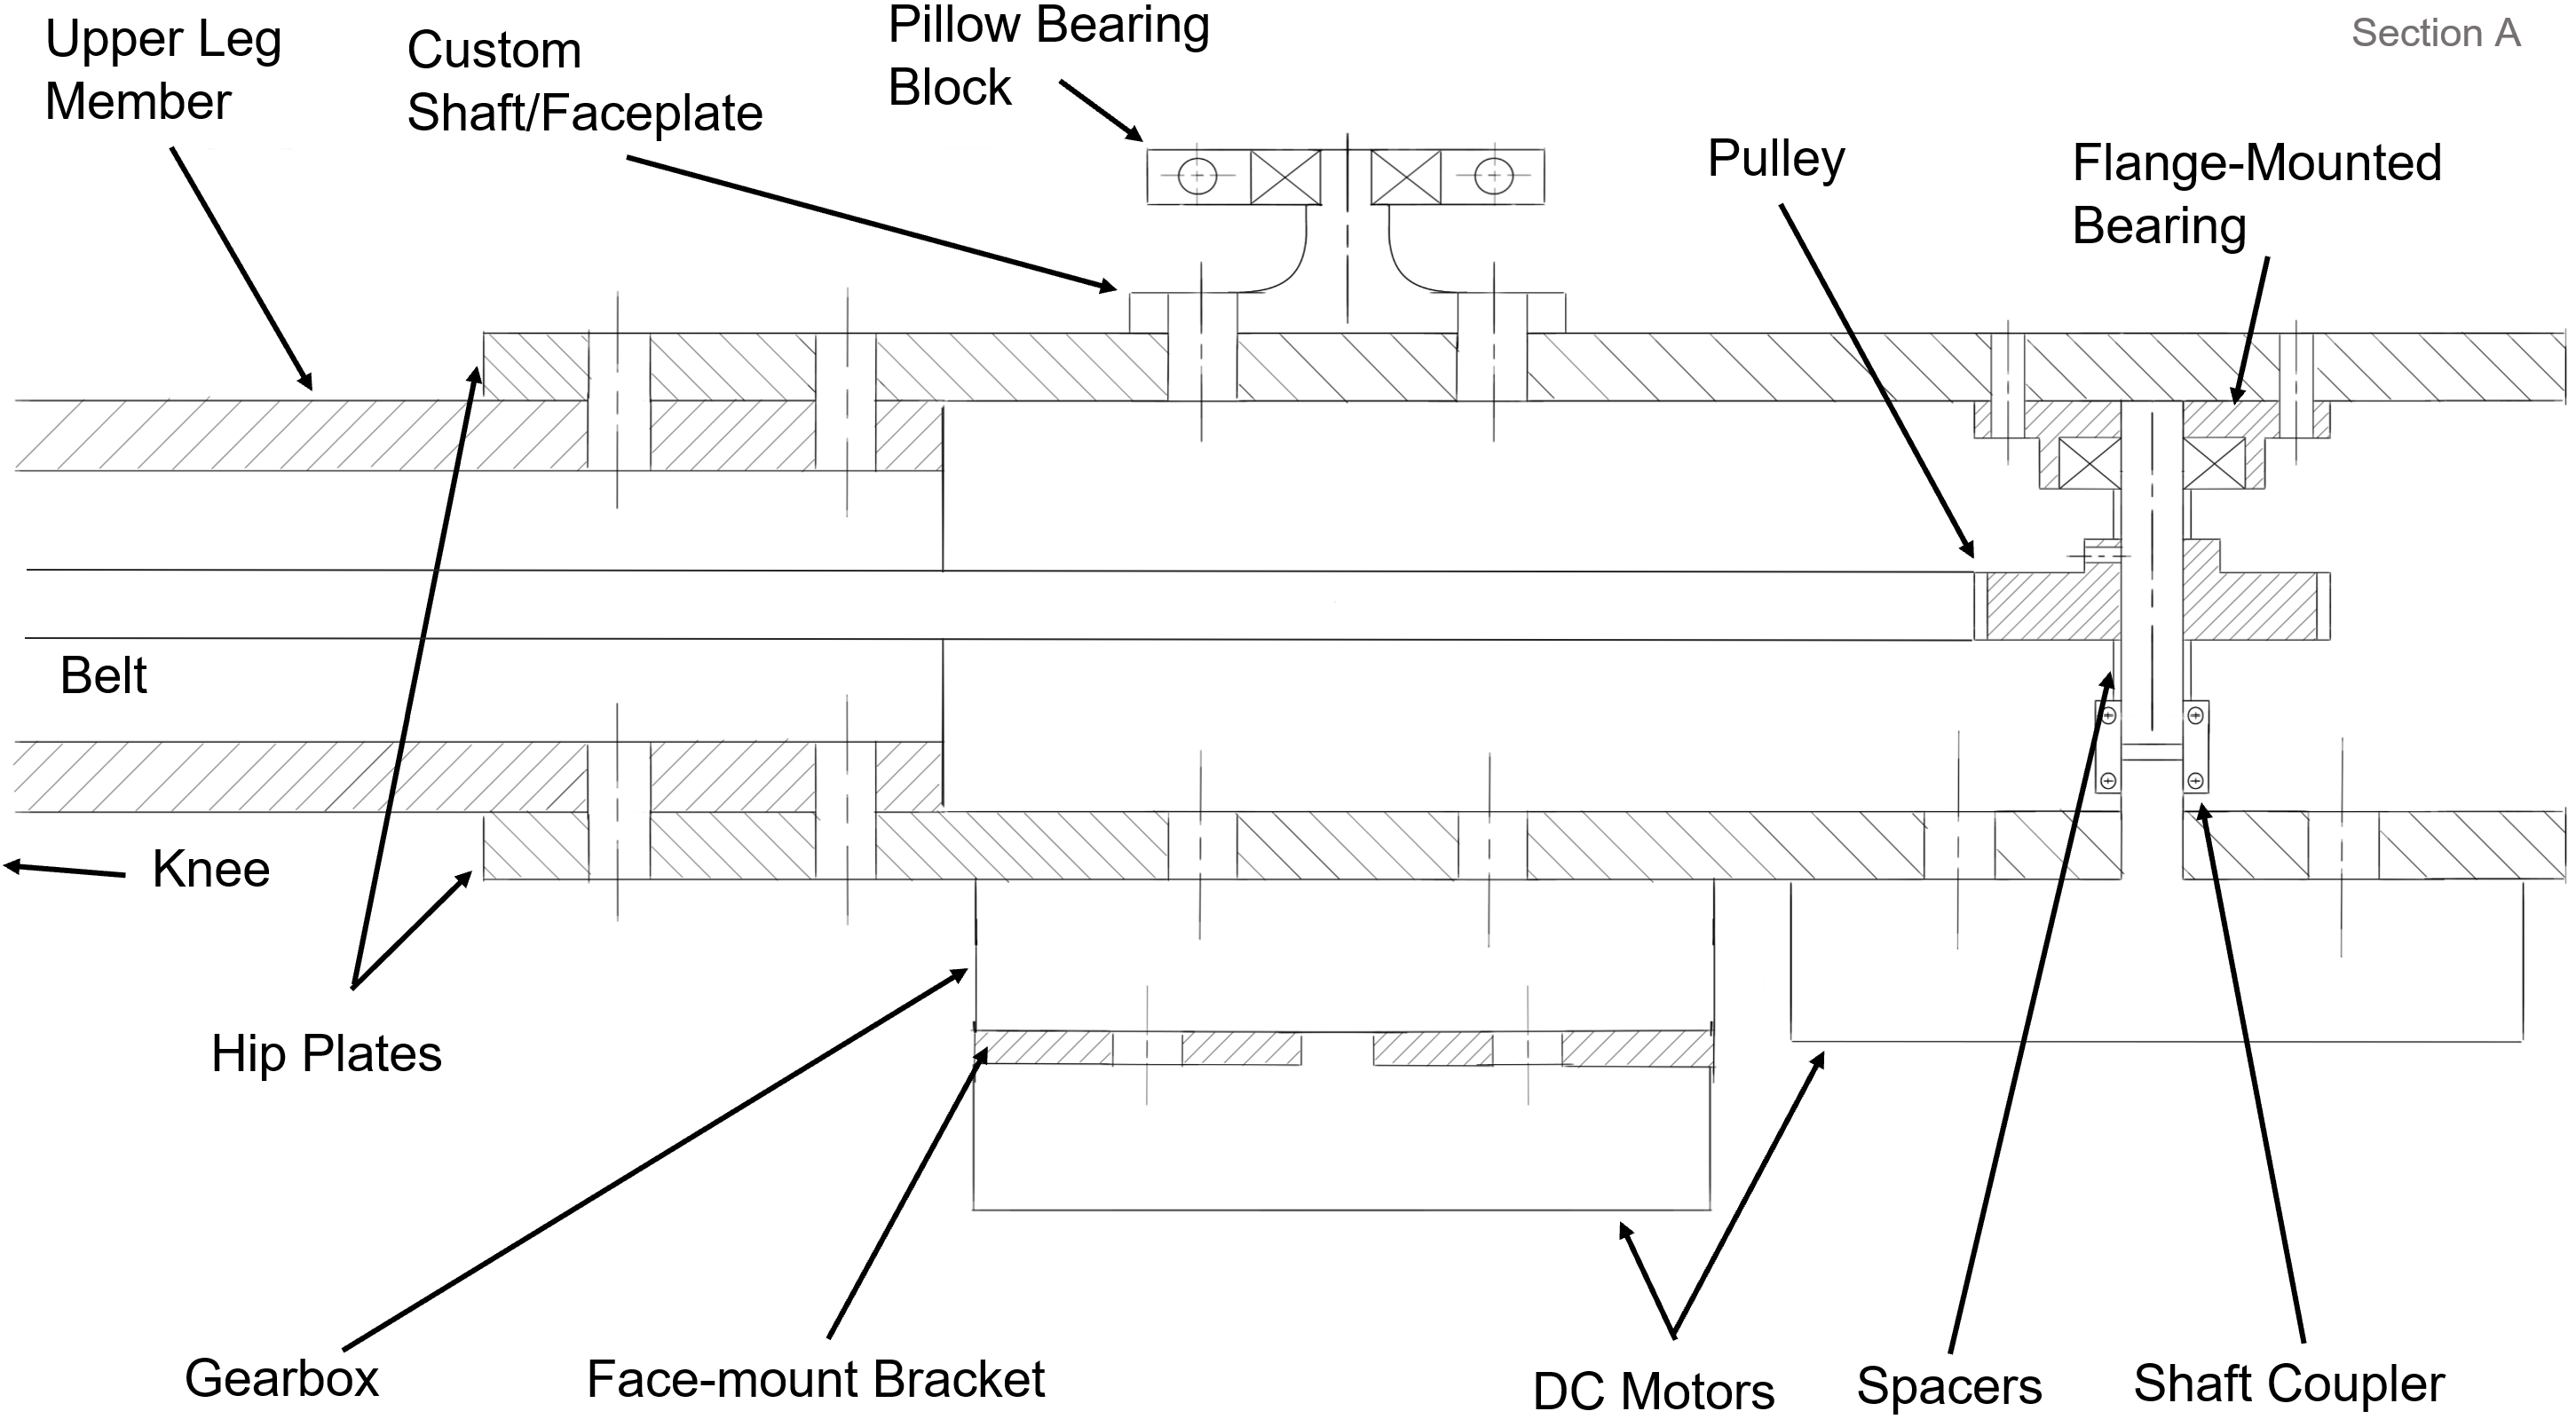
\includegraphics[width=0.8\textwidth]{3_DesignConcepts/img/Crab/crab_hip.png}
    \caption{Crab Top Section View (Section A) - Leg and Hip}
    \label{fig:crab_hip}
\end{figure}

\begin{figure}[H]
    \centering
    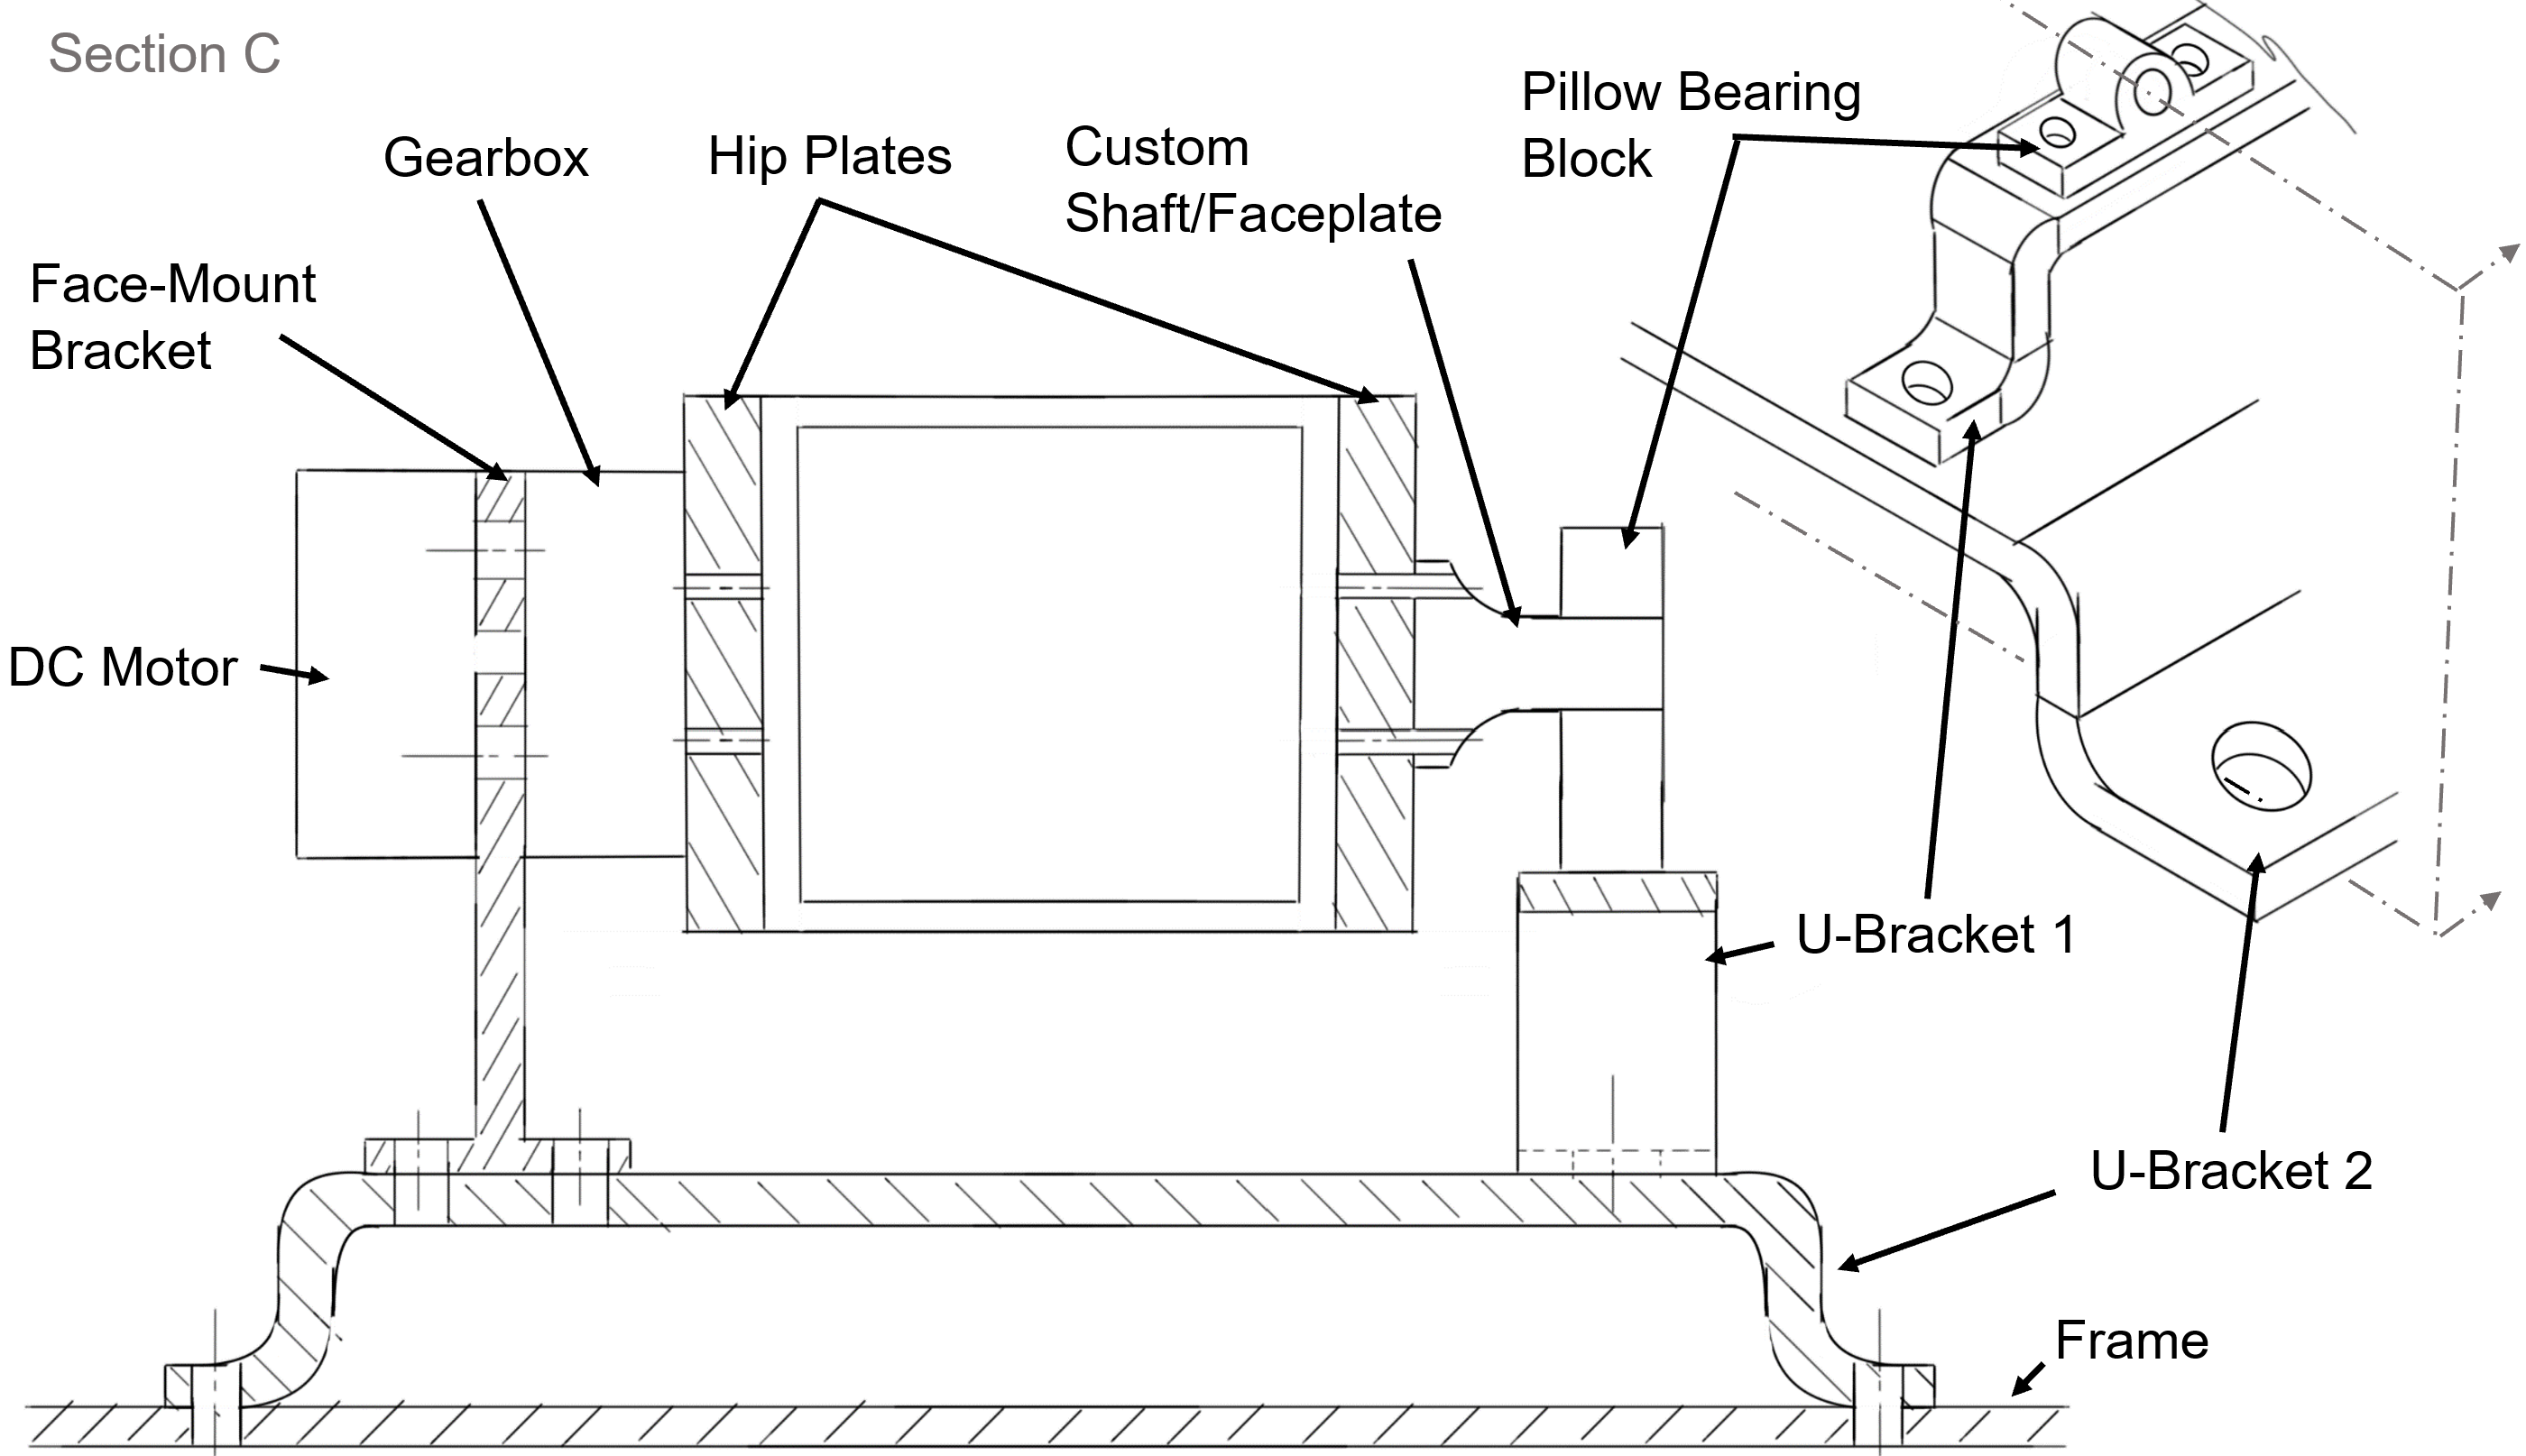
\includegraphics[width=0.8\textwidth]{3_DesignConcepts/img/Crab/crab_hip_cut.png}
    \caption{Crab Side Section View (Section C) - U-bracket Mounting}
    \label{fig:crab_hip_cut}
\end{figure}

A detailed concept of the knee joint (Section B as per Figure \ref{fig:crab_leg}) is shown in Figure \ref{fig:crab_knee}. It consists of a pulley (driven by one of the motors in the hip) which is directly fastened onto the lower shin linkage. The pulley is free to move on the shaft, which is supported by flange hub bearings on the thigh linkage. For this reason, no hub mount was drawn for this pulley, however in further design it may be required to add one to reduce the shaft size. In this case, a spacer would be added on the other side of the pulley to keep balance between the two sides. The knee can be easily assembled due to the simple shaft and the fastened side plates on the thigh linkage. 

\begin{figure}[H]
    \centering
    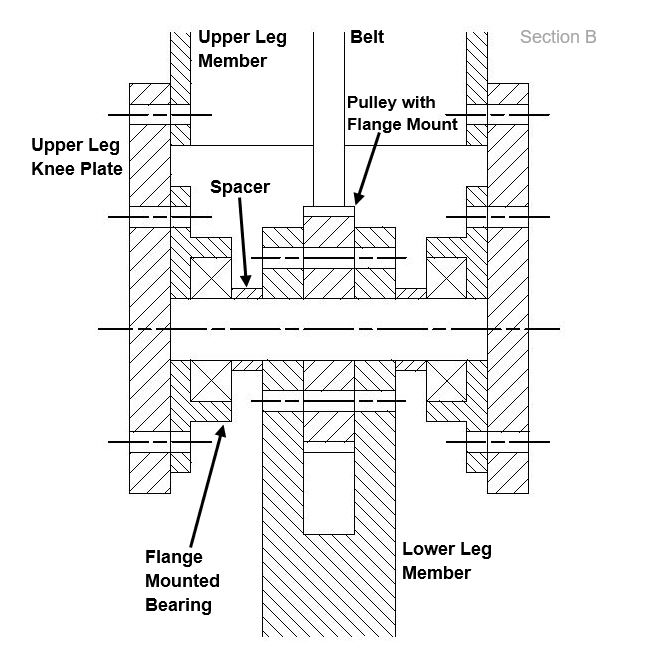
\includegraphics[width=0.8\textwidth]{3_DesignConcepts/img/Crab/crab_knee.JPG}
    \caption{Crab Top Section View (Section B) - Leg and Knee}
    \label{fig:crab_knee}
\end{figure}

Figure \ref{fig:crab_foot} shows the foot design for the crab. It consists of a molded flexible silicon piece which can be slipped onto the shin linkage and is retained by a protruding ridge.

\begin{figure}[H]
    \centering
    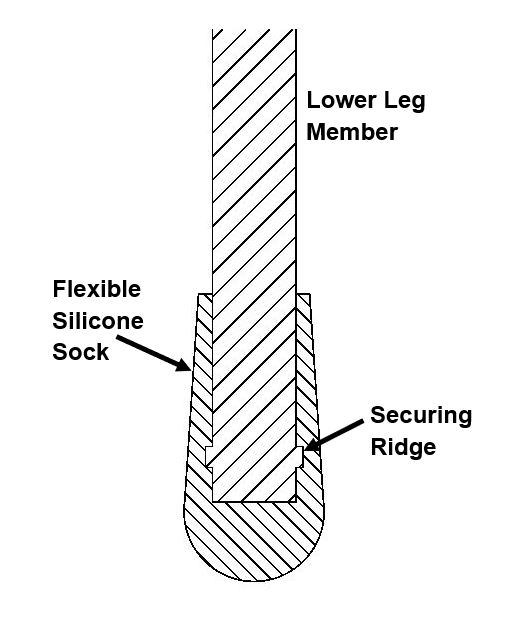
\includegraphics[width=0.5\textwidth]{3_DesignConcepts/img/Crab/crab_foot.JPG}
    \caption{Crab Side View - Leg and Foot}
    \label{fig:crab_foot}
\end{figure}

A possible configuration for the weatherproofing and accessibility of the chassis is shown in Figure \ref{fig:crab_chassis}. A hinge is used on one side to facilitate access to the inside components for maintenance. A flange-type gasket is included all around the chassis to seal the "lid". It is secured by bolts. 

\begin{figure}[H]
    \centering
    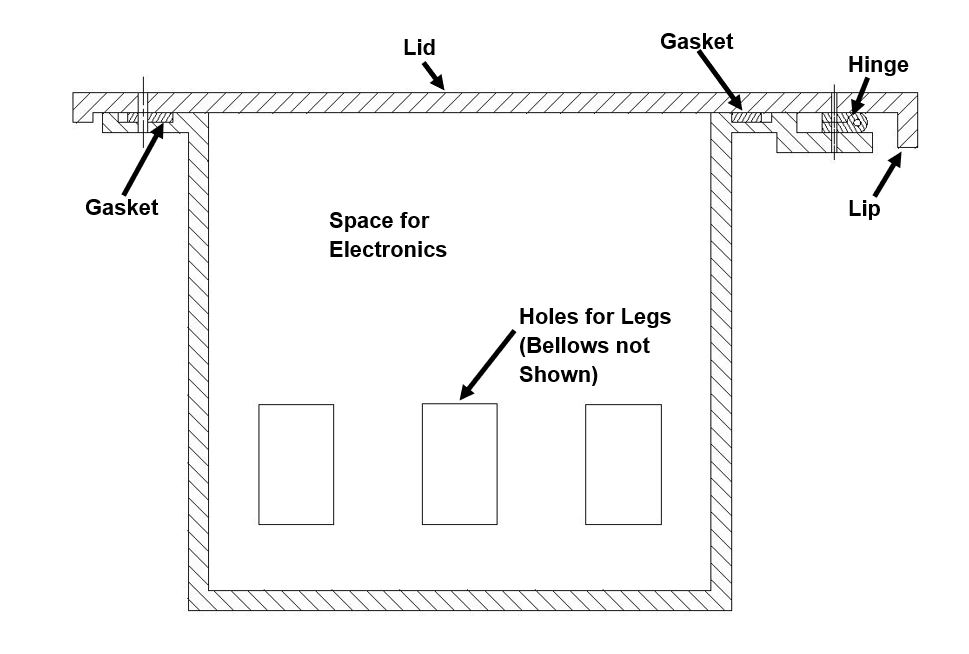
\includegraphics[width=0.8\textwidth]{3_DesignConcepts/img/Crab/crab_chassis.JPG}
    \caption{Crab Side View - Chassis}
    \label{fig:crab_chassis}
\end{figure}



%------------------------- CONCEPT 3 -------------------------%
\subsection{Concept 3 - Spider}

The third concept, shown in Figure \ref{fig:spider_over}, is based on a spider-like leg morphology. Six legs provide superior stability to four; each leg has three degrees of freedom, allowing it to rotate and lift at the hip, as well as extend at the knee \cite{robot_platform_robot_nodate}. Round flange-mounted bellows are used to seal the joints from water, dust, amongst others. The leg linkages are made out of I-beams for structural rigidity.
Figure \ref{fig:spider_over} also shows the location of the various electrical components. These are positioned onto mounting plates inside the chassis. A front view of the chassis is also shown in Figure \ref{fig:spider_frame_front}.

\begin{figure}[H]
    \centering
    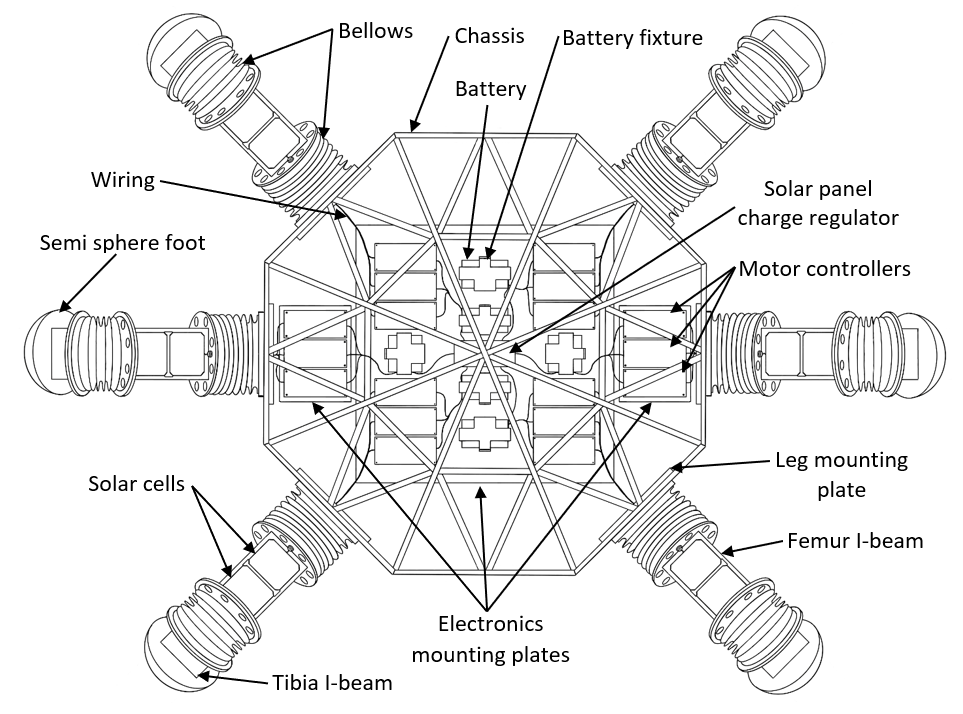
\includegraphics[width=\textwidth]{3_DesignConcepts/img/C3/overview_ann.PNG}
    \caption{Spider Top View - Overview}
    \label{fig:spider_over}
\end{figure}


\begin{figure}[H]
    \centering
    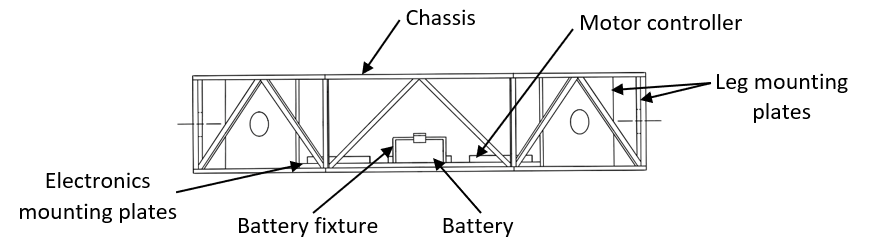
\includegraphics[width=0.9\textwidth]{3_DesignConcepts/img/C3/framefront_ann.PNG}
    \caption{Spider Front View - Frame}
    \label{fig:spider_frame_front}
\end{figure}

A detailed drawing of the knee joint is shown in Figure \ref{fig:spider_knee}. There are plate discs mounted onto the end of the I-beams to help in the mounting of components. They provide easy mounting points for the bellow flanges. Support plates for the motor are then added using L-brackets. The motor has a shaft that extends on both other ends, which allows it to be supported on both sides and balances the forces acting on the motor. The motor then is face mounted onto the multi-stage planetary gearbox. Only one of the motor shafts is attached to the gearbox and fixed to the lower link to move it with a flange collar. The other side is simply floating in bearings.

\begin{figure}[H]
    \centering
    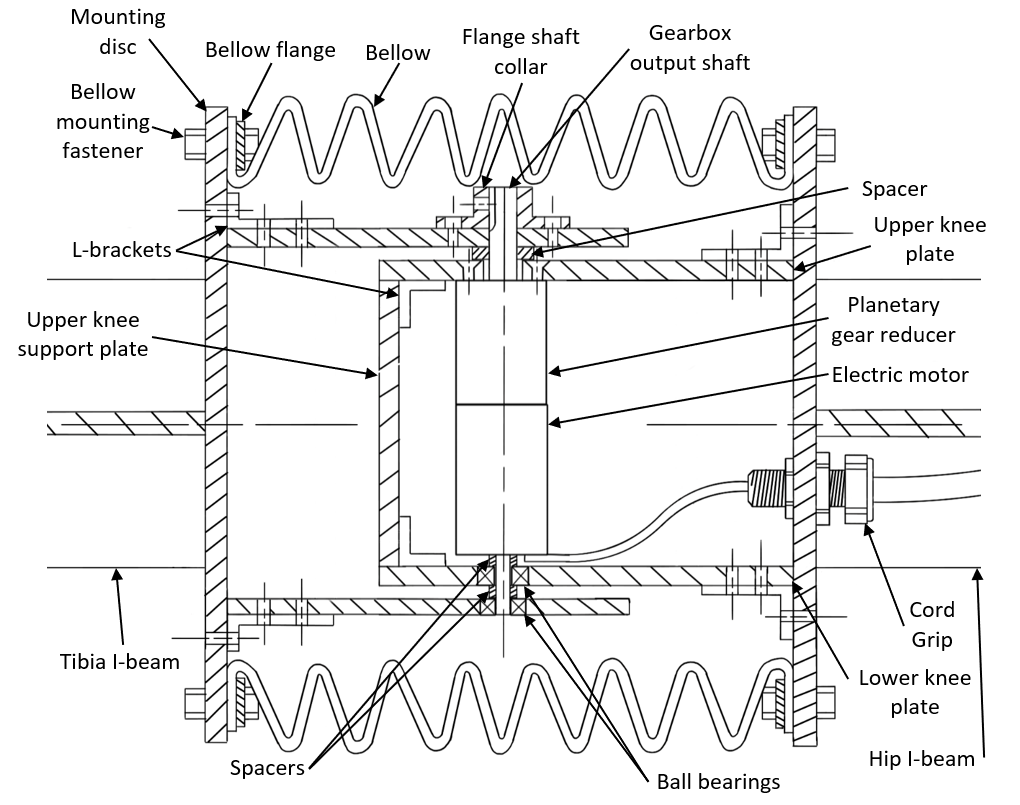
\includegraphics[width=\textwidth]{3_DesignConcepts/img/C3/kneejoint_ann.PNG}
    \caption{Spider Top View - Knee Joint}
    \label{fig:spider_knee}
\end{figure}

The hip joint, shown in Figure \ref{fig:spider_hip}, uses similar principles to the knee joint. However, there are two motors positioned perpendicularly by U-shaped brackets, which allows for two degrees of freedom at the hip. Cord grips are used to feed the cables from the knee joints to the chassis for a waterproof design. The hip joint is mounted onto the chassis using longer bolts and a mounting plate positioned inside the chassis. A gasket is also used to seal the joint from the environment. Also, corner-mount draw latches are mounted at each edge of the octagon upper casing for a quick connection with the lower casing.

\begin{figure}[H]
    \centering
    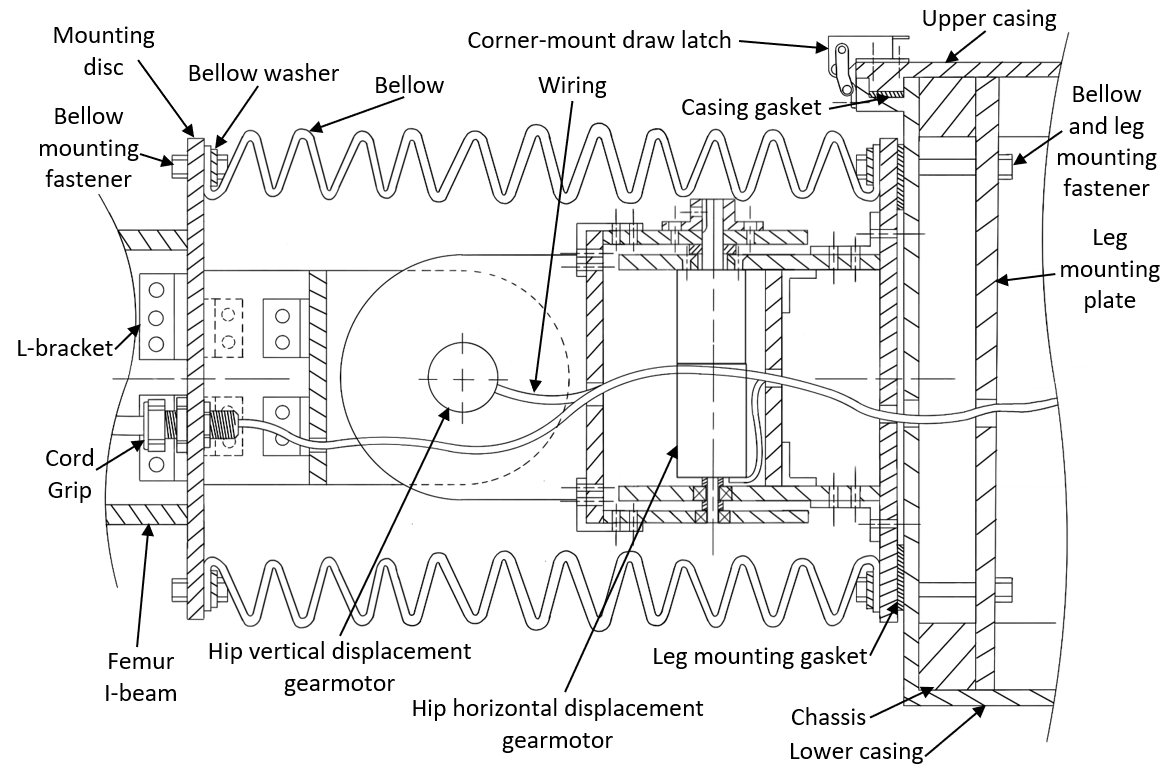
\includegraphics[width=\textwidth]{3_DesignConcepts/img/C3/hipjoint_ann.PNG}
    \caption{Spider Front View - Hip Joint}
    \label{fig:spider_hip}
\end{figure}

%------------------------- SOLAR PANEL -------------------------%
\subsection{Solar Panel Concepts}

Three solar panel concepts were created to explore various configurations. The concepts were not created based on any specific robot/locomotion concept as seen previously. Instead, they were made with the intention that they could be accommodated on those designs easily or with minor changes. The major goal was to explore options to maximize solar panel surface area, and consequently maximize power. 


\subsubsection{Concept 1 - Solar Roof}

The solar roof, as shown in Figure \ref{fig:solar_roof} consists in a light hollow tube structure with a curved sheet on top, on which a flexible solar panel is fastened using its grommets and some bolts. The curved surface that droops over the sides of the robot allows for maximum surface area. The solar panel is also elevated away from the robot, making it less likely to interfere with the waste collection system and legs.
The structure consists of four side support beams (2 per side) bolted on the curved sheet and the side of the chassis. It also has two crossed beam structures bolted on top of the chassis, with the curved sheet simply resting on top.

\begin{figure}[H]
    \centering
    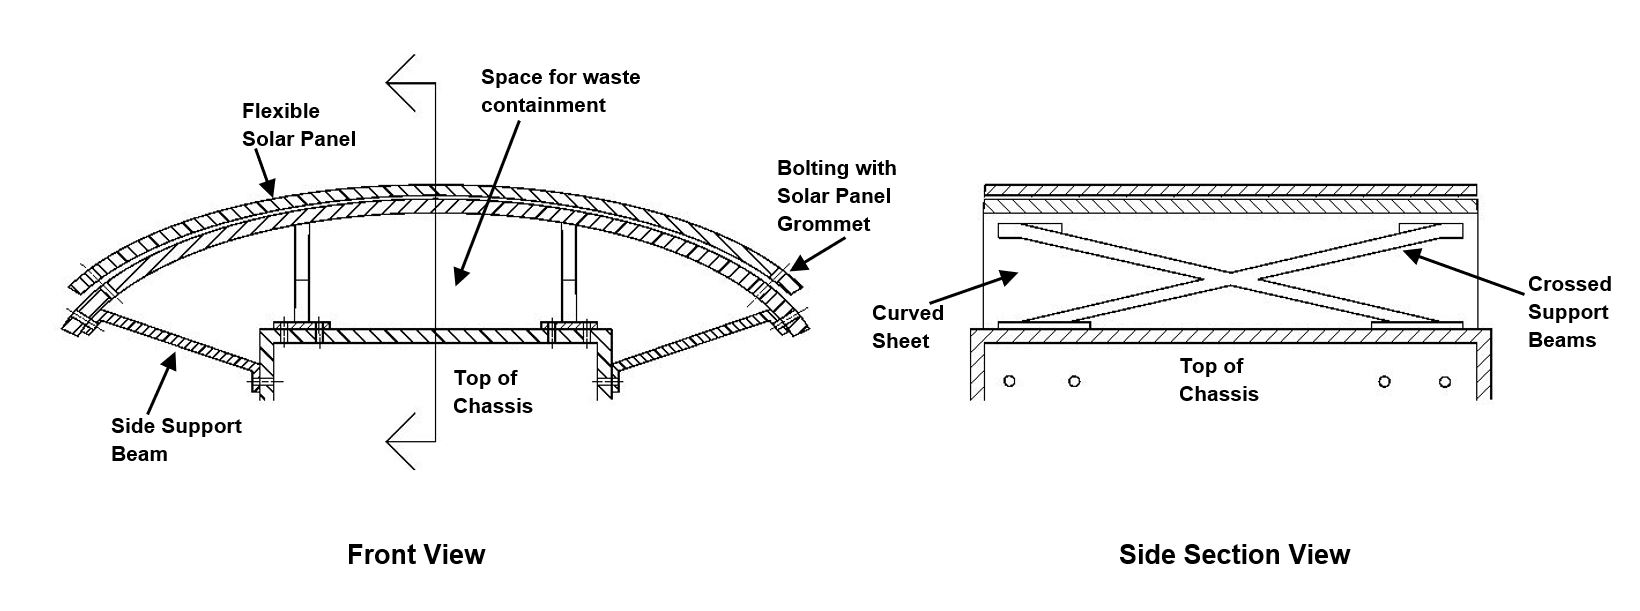
\includegraphics[width=\textwidth]{3_DesignConcepts/img/Solar/solar_roof.JPG}
    \caption{Solar roof concept}
    \label{fig:solar_roof}
\end{figure}

\subsubsection{Concept 2 - Solar Awning}

The solar awning, as shown in Figure \ref{fig:solar_sidePanel}, allows easy compatibility with any garbage picker concept requiring access to the roof of the robot. The concept uses typical metal stud tracks and wall angle channels as structural support for the solar panels. The metal studs are mounted using regular fasteners such as bolts on the side of the robot's chassis or casing/shell. The flexible solar panel is secured onto the studs using grommets and bolts.

\begin{figure}[H]
    \centering
    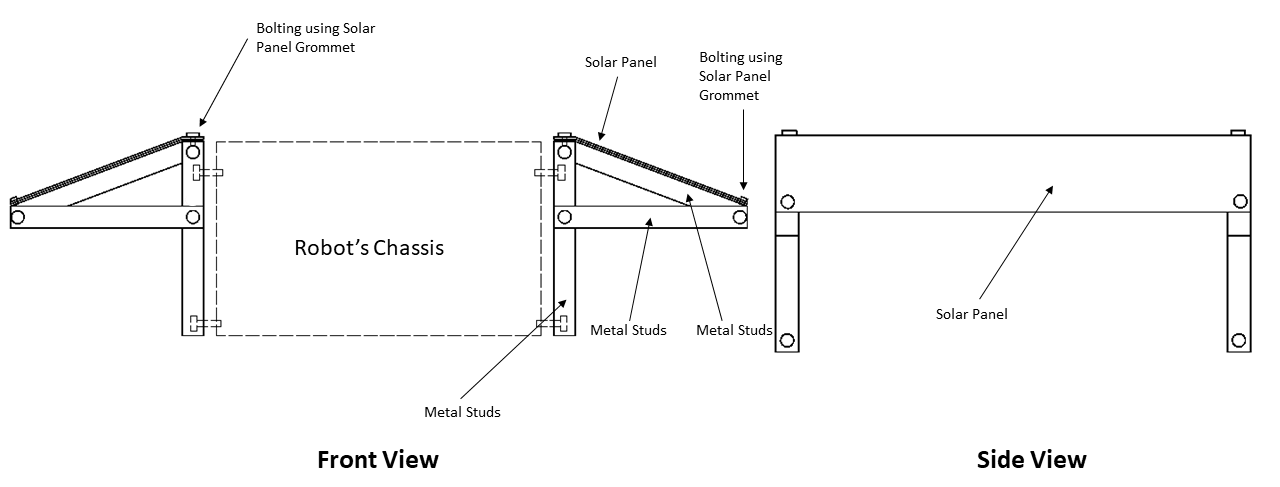
\includegraphics[width=0.9\textwidth]{img/Solar/SolarSidePanel.png}
    \caption{Solar awning concept}
    \label{fig:solar_sidePanel}
\end{figure}


\subsubsection{Concept 3 - Solar Cells}

The third option is installing the solar cells onto the robot chassis and legs themselves with adhesive, as shown in Figure \ref{fig:solarcells} \cite{gioco_solutions_installation_2018} \cite{3m_3m_nodate}. The useful area is whatever surfaces are exposed on the robot.
A possible downside of this design is that depending on the form-factor of the litter collecting unit, the amount of space available for solar cells on the chassis may be limited.
If the collector is in the form of a cube, then there is useful area on the top.
Other shapes may provide less space for mounting solar cells.
Additionally, increasing the width of leg linkages to accept solar cells will also increase the weight of the linkage, increasing the overall weight and power consumption.

\begin{figure}[H]
    \centering
    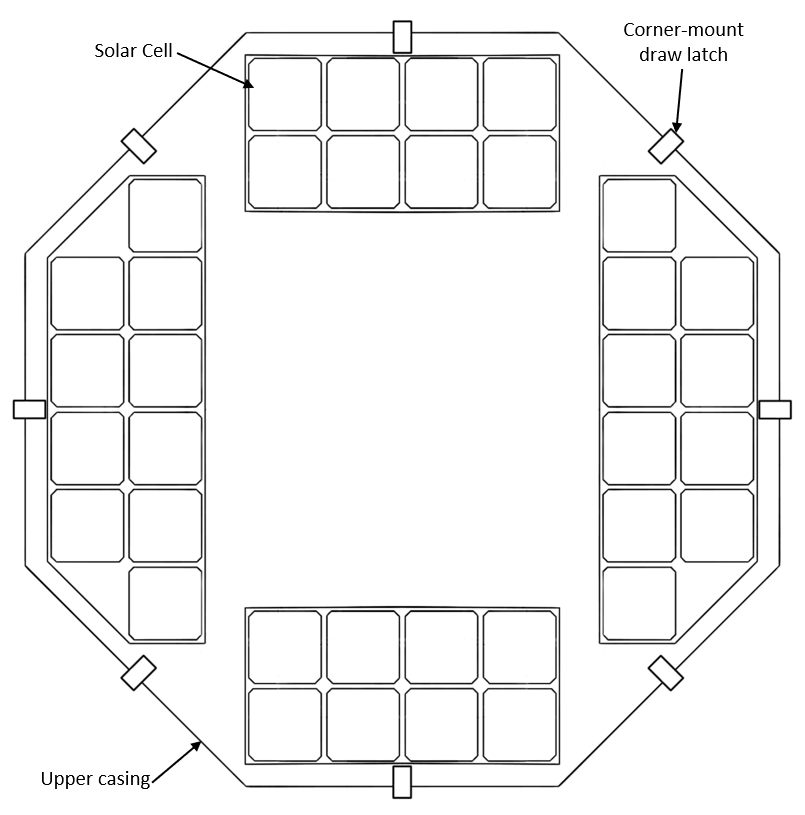
\includegraphics[width=0.8\textwidth]{3_DesignConcepts/img/C3/solarcells_ann.PNG}
    \caption{Custom solar cell positioning concept}
    \label{fig:solarcells}
\end{figure}